\section{Variational Classical Networks}
    \begin{frame}[t]
        \frametitle{Why and How should Parameters be variational?}

        \vspace{-0.6cm}
        \begin{columns}[t]
            \column{0.4\textwidth}
                \begin{itemize}
                    \item Theoretically: always better approximation through higher order terms \pause
                    \begin{itemize}
                        \item Hard to calculate analytically and expensive to evaluate \pause
                    \end{itemize}
                    \item Hope: Better behavior if parameters are \emph{learned}/\emph{optimized}, starting from the analytical result \pause
                \end{itemize}
    
            \column{0.4\textwidth}
                \vspace{-0.3cm}
                \makebox[\textwidth][c]{
                    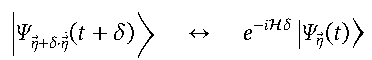
\includegraphics[width=0.95\textwidth,page=1]{main-content/variational-classical-networks/variational-classical-networks-theory.pdf}
                }
                \pause
                \makebox[\textwidth][c]{
                    \includegraphics[width=0.7\textwidth,page=2]{main-content/variational-classical-networks/variational-classical-networks-theory.pdf}
                }%
                \pause
                \vspace{1cm}
                \makebox[\textwidth][c]{
                    \includegraphics[width=1.1\textwidth,page=3]{main-content/variational-classical-networks/variational-classical-networks-theory.pdf}
                }
                \pause
                \makebox[\textwidth][c]{
                    \includegraphics[width=0.7\textwidth,page=4]{main-content/variational-classical-networks/variational-classical-networks-theory.pdf}
                }
    
        \end{columns}
        
        % notes 
        \onslide % on all slides of frame
        \note[item] {
            Time dependent variational principle (TDVP)
        }
        \note[item] {
            Variational classical network (VCN)
        }
    \end{frame}


    \begin{frame}[t]
        \frametitle{Why and How should Parameters be variational?}

        \vspace{-0.6cm}
        \begin{columns}[t]
            \column{0.4\textwidth}
                \begin{itemize}
                    \item Theoretically: always better approximation through higher order terms
                    \begin{itemize}
                        \item Hard to calculate analytically and expensive to evaluate
                    \end{itemize}
                    \item Hope: Better behavior if parameters are \emph{learned}/\emph{optimized}, starting from the analytical result
                \end{itemize}
    
            \column{0.4\textwidth}
                \vspace{-0.3cm}
                \makebox[\textwidth][c]{
                    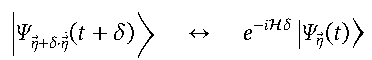
\includegraphics[width=0.95\textwidth,page=1]{main-content/variational-classical-networks/variational-classical-networks-theory.pdf}
                }
                \makebox[\textwidth][c]{
                    \includegraphics[width=0.7\textwidth,page=2]{main-content/variational-classical-networks/variational-classical-networks-theory.pdf}
                }%
                \pause
                \vspace{0.5cm}
                \makebox[\textwidth][c]{
                    \includegraphics[width=1.1\textwidth,page=5]{main-content/variational-classical-networks/variational-classical-networks-theory.pdf}
                }%
                \pause
                \vspace{0.15cm}
                \makebox[\textwidth][c]{
                    \includegraphics[width=0.6\textwidth,page=6]{main-content/variational-classical-networks/variational-classical-networks-theory.pdf}
                }
    
        \end{columns}
        
        % notes 
        \onslide % on all slides of frame
        \note[item] {
            Pseudo inversion
        }
    \end{frame}

    \begin{frame}[t]
        \frametitle{First Try: Cumulant Expansion Prefactors}

        \begin{itemize}
            \item Idea: generate a variational Hamiltonian by replacing the analytical prefactors
        \end{itemize}
        \vspace{-0.2cm}
        \makebox[\textwidth][c]{
            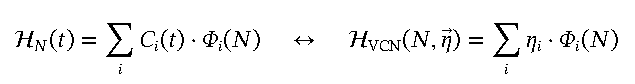
\includegraphics[width=0.7\textwidth,page=1]{main-content/variational-classical-networks/variational-classical-networks-application.pdf}
        }%
        \vspace{0.4cm}
        \pause
        \makebox[\textwidth][c]{
            \hspace{-1.5cm}
            \makebox[0.5\textwidth][c]{
                \includegraphics[width=0.5\textwidth,page=2]{main-content/variational-classical-networks/variational-classical-networks-application.pdf}%
            }
            \makebox[0.5\textwidth][c]{
                \raisebox{0.55cm}{
                    \includegraphics[width=0.5\textwidth,page=3]{main-content/variational-classical-networks/variational-classical-networks-application.pdf}
                }
            }
        }
        
        % notes 
        \onslide % on all slides of frame
        \note[item] {
            TODO
        }
    \end{frame}

    \begin{frame}[t]
        \frametitle{Correction: Watch Explicit Time-Dependency}

        \begin{itemize}
            \item First strategy is not suitable
            \begin{itemize}
                \item Energy- and variance is not conserved
            \end{itemize}
            \pause
            \item Problem: explicit time-dependency of base energy
        \end{itemize}

        \makebox[\textwidth][c]{
            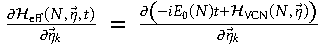
\includegraphics[width=0.55\textwidth,page=1]{main-content/variational-classical-networks/variational-classical-networks-application-explicit.pdf}
        }

        \pause
        \begin{itemize}
            \item Solution: Replace base energy factors with variational parameters
        \end{itemize}

        \makebox[\textwidth][c]{
            \includegraphics[width=0.3\textwidth,page=3]{main-content/variational-classical-networks/variational-classical-networks-application-explicit.pdf}
            \raisebox{1cm}{
                \includegraphics[width=0.62\textwidth,page=2]{main-content/variational-classical-networks/variational-classical-networks-application-explicit.pdf}
            }
        }
        
        % notes 
        \onslide % on all slides of frame
        \note[item] {
            TODO
        }
    \end{frame}
